\begin{figure*}
\centering

\begin{subfigure}{\textwidth}

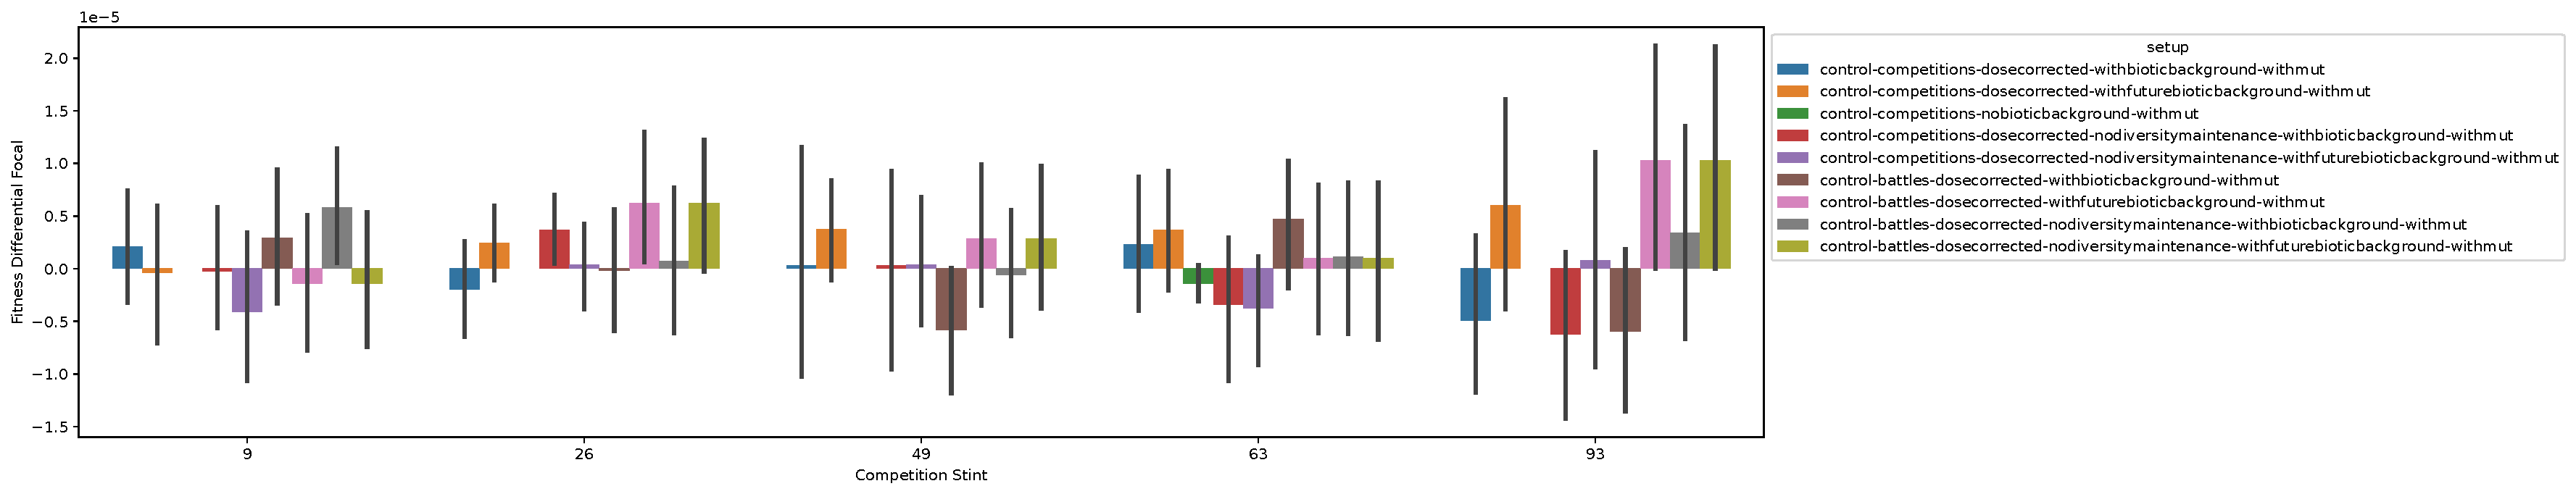
\includegraphics[width=\linewidth]{{submodule/dishtiny/binder/bucket=prq49/a=adaptation_assays+endeavor=16/teeplots/hue=setup+viz=barplot+x=competition-stint+y=fitness-differential-focal+ext=}}
\caption{
Calculated fitness differential between competing strains based on population composition at the end of competition experiments.
Zero is neutral.
Error bars are 95\% confidence intervals.
}
\end{subfigure}

\begin{subfigure}{\textwidth}
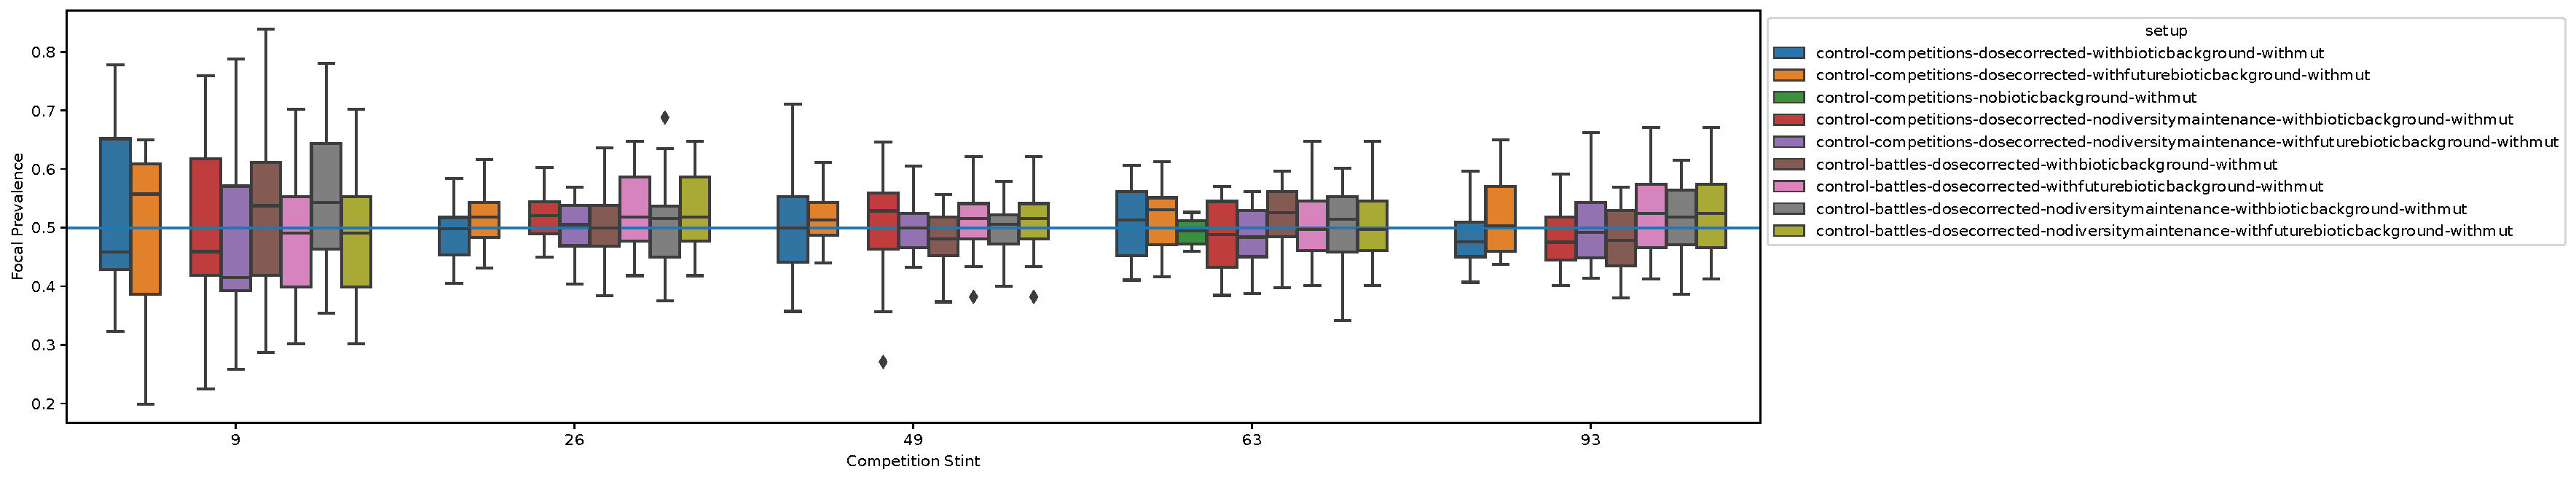
\includegraphics[width=\linewidth]{{submodule/dishtiny/binder/bucket=prq49/a=adaptation_assays+endeavor=16/teeplots/hue=setup+viz=boxplot+x=competition-stint+y=focal-prevalence+ext=}}
\caption{
Fractional composition of focal population at the end of competition experiments.
A neutral outcome corresponds to even (0.5) composition, annotated with a horizontal line.
}
\end{subfigure}

\begin{subfigure}{\textwidth}
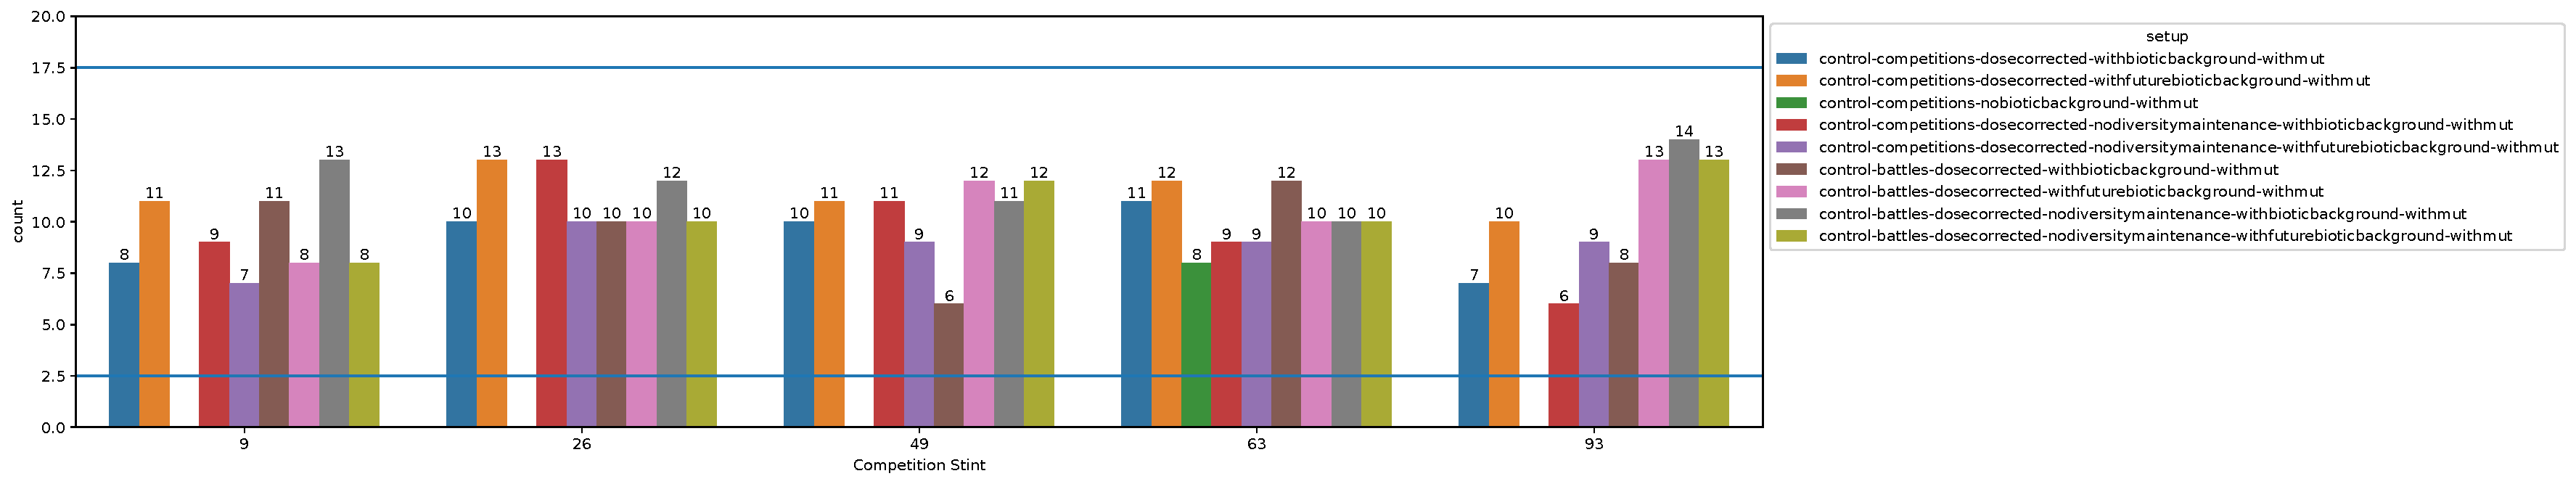
\includegraphics[width=\linewidth]{{submodule/dishtiny/binder/bucket=prq49/a=adaptation_assays+endeavor=16/teeplots/hue=setup+viz=countplot+x=competition-stint+ext=}}
\caption{
Number competitions out of 20 won by first strain.
Ten competitions won corresponds to a perfectly neutral outcome.
Eighteen and more or two or less competitions won were considered to indidicate a significant fitness difference between strains.
These thresholds for significance annotated with horizontal lines.
}
\end{subfigure}

\caption{
Control adaptation experiments for selected stints.
Control experiments were performed by competing two identical genomes or populations against each other with the contemporary biotic background, with the prefatory biotic background, or with no biotic background.
See Figure \ref{fig:adaptation_assay_cartoon} for summary of adaptation experiment design.
}
\label{fig:adaptation_control}
\end{figure*}
